\chapter{Architektur Übersicht}
\label{chap:Architektur-Übersicht}

\begin{figure}[ht]
  \centering
  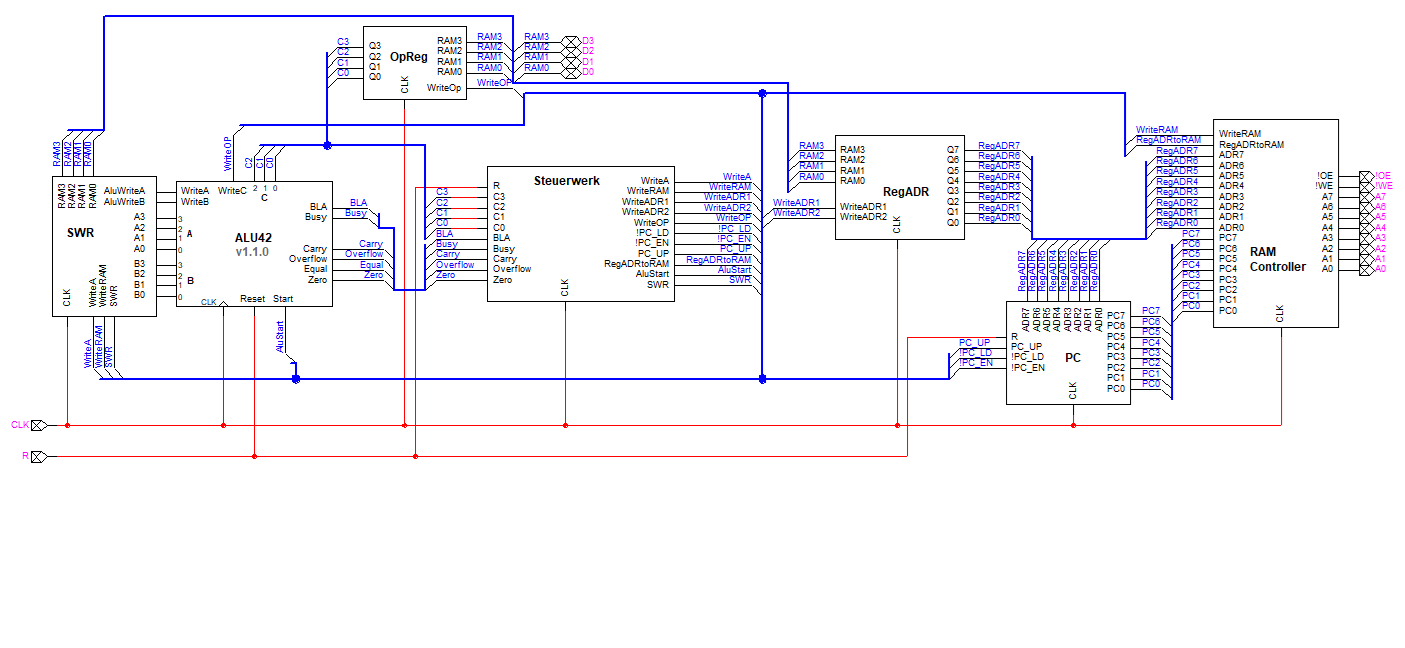
\includegraphics[scale=0.5]
  {content/figures/Blockschaltbild-steuerwerk-innen.png}
  \caption{LogicWorks Blockschaltbild Steuerwerk}
  \label{fig:lw-bsb-steuerwerk}
\end{figure}


\begin{figure}[ht]
  \centering
  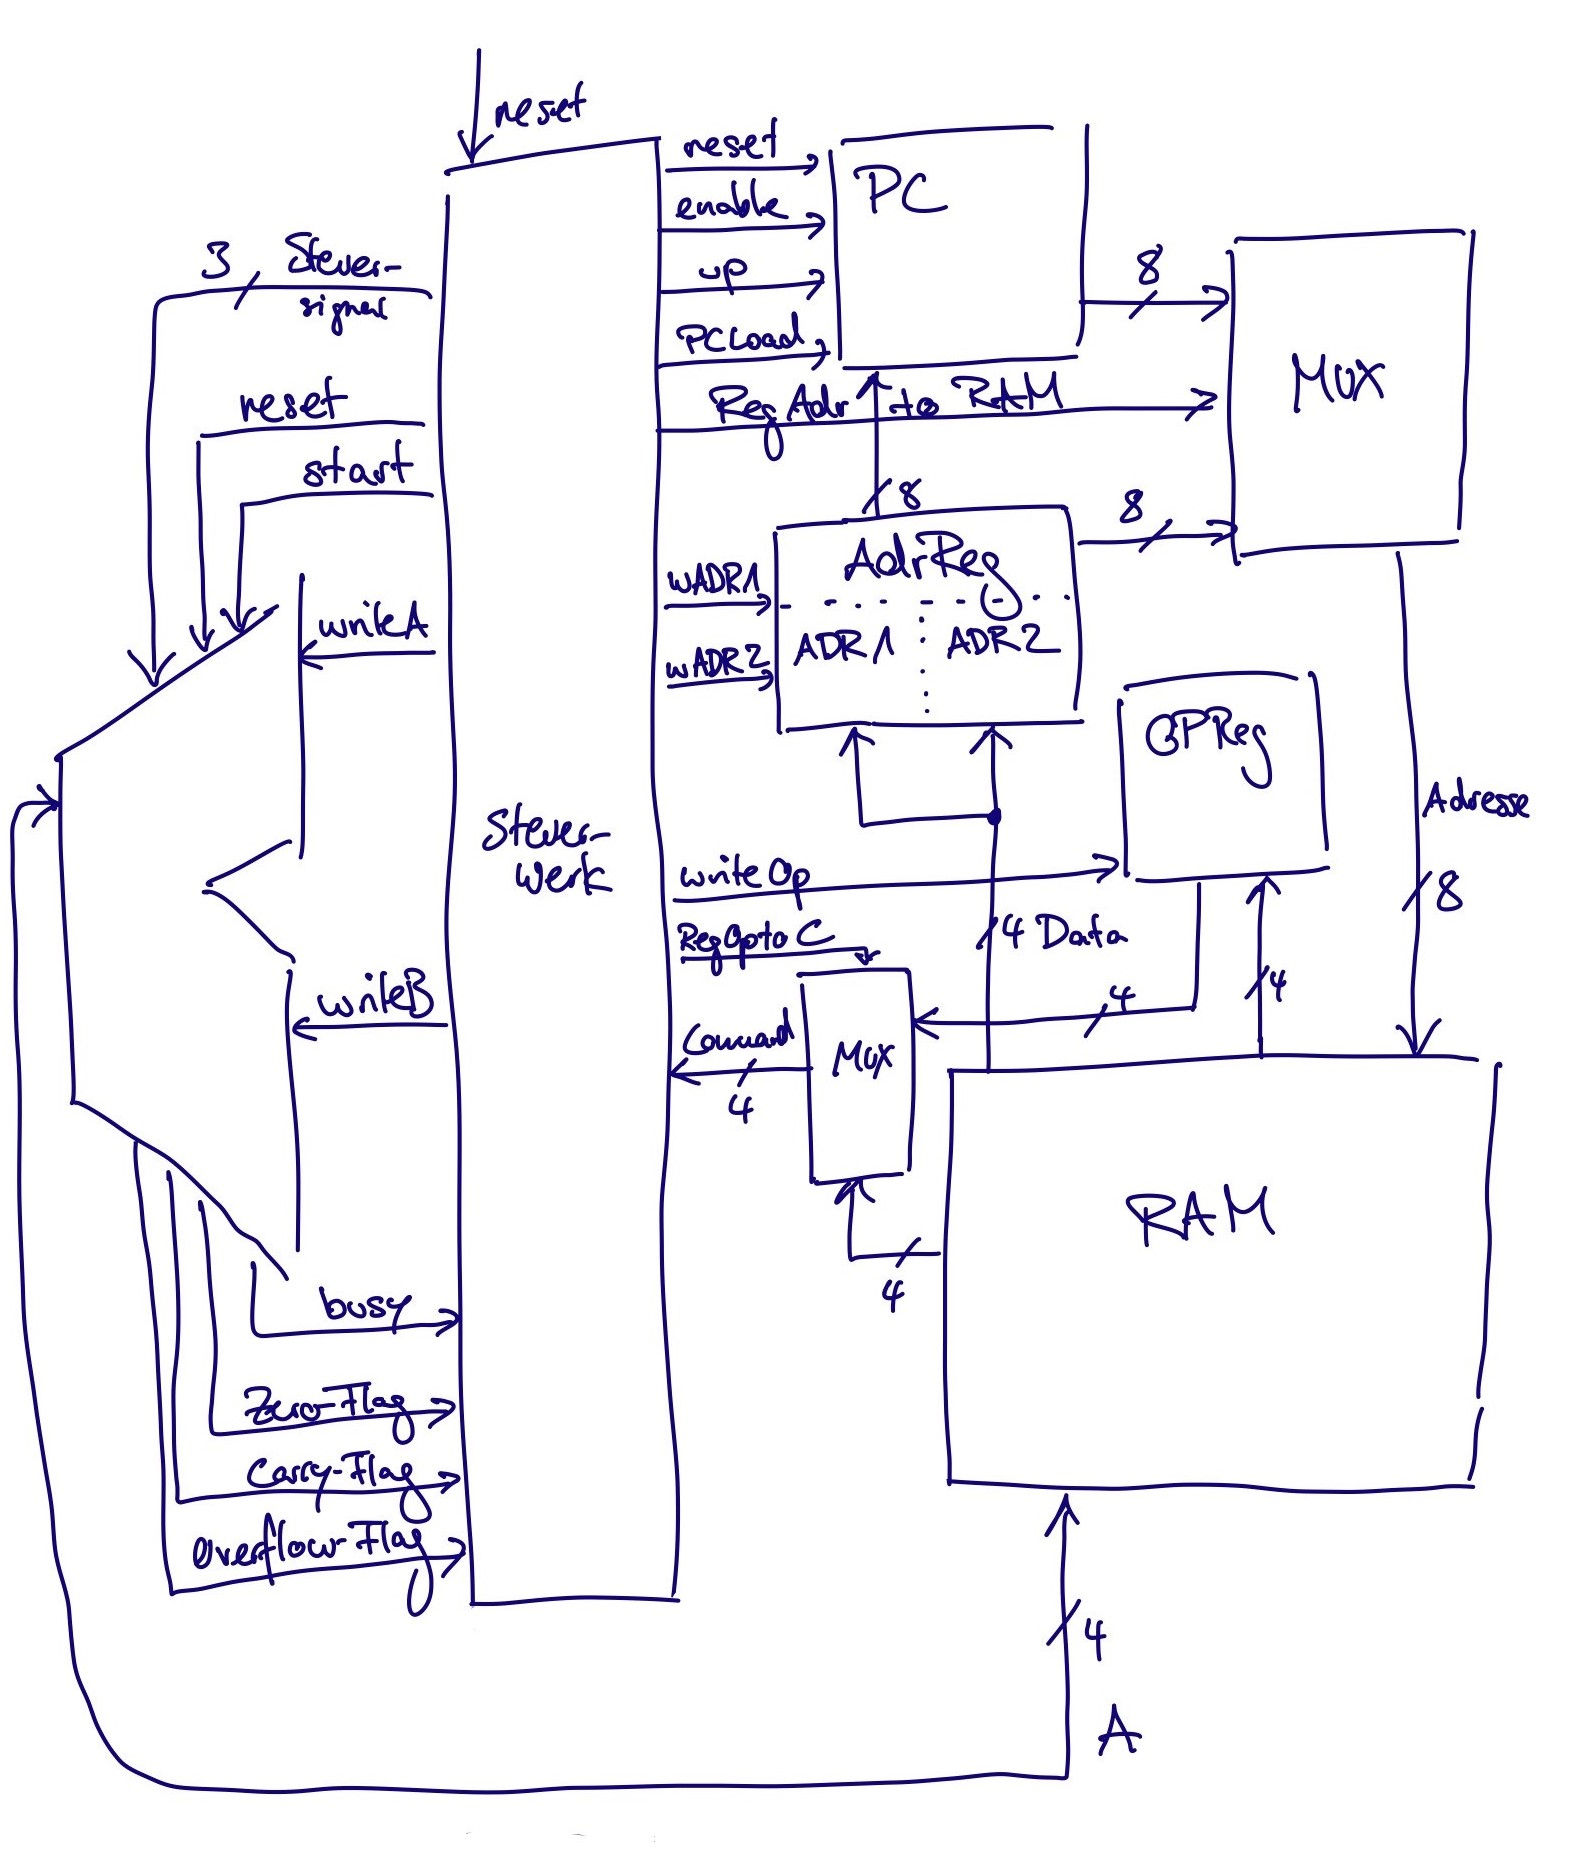
\includegraphics[scale=0.3]
  {content/figures/BSB_SW.jpg}
  \caption{First Level Blockschaltbild}
  \label{fig:blockschaltbild-first-level}
\end{figure}

\subsection{Transitionsfunktion Überführungsfunktion}
\label{sec:transitionsfunktion}

\begin{figure}[ht]
  \centering
  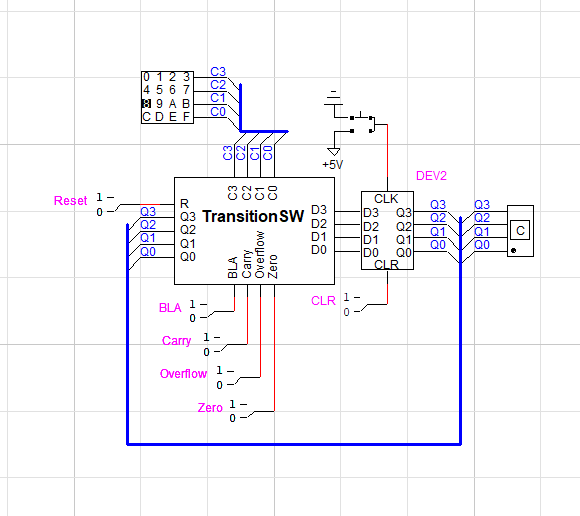
\includegraphics[scale=0.6]
  {content/figures/Transitionsfunktion.png}
  \caption{Blockschaltbild der Transitionsfunktion}
  \label{fig:blockschaltbild-transitionsfunktion}
\end{figure}

\begin{figure}[ht]
  \centering
  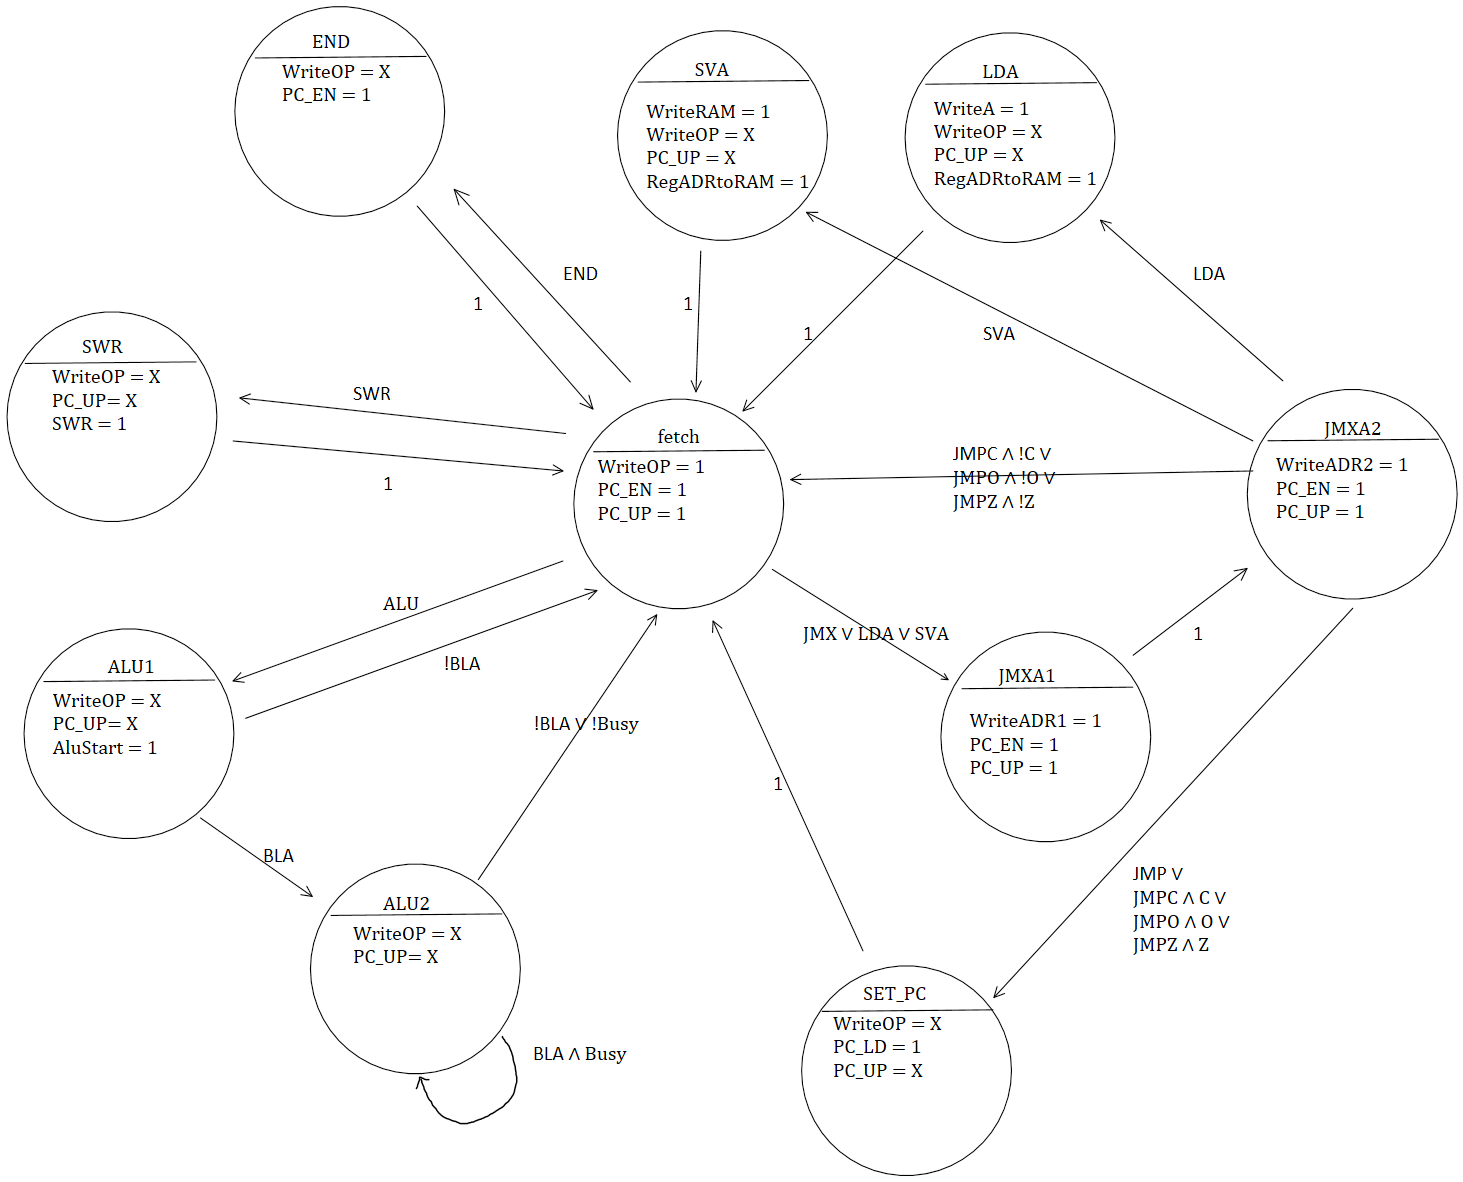
\includegraphics[scale=0.279]
  {content/figures/SW_Zustaende}
  \caption{Zustandsautomat Steuerwerk}
  \label{fig:SW_Zustaende}
\end{figure}

\subsection{Steuerwerk Ein und Ausgänge}
\label{sec:steuerwerk-ein-und-ausgänge}

\textbf{Eingänge}
\begin{itemize}
  \item Reset
  \item Q3..0
  \item BLA (Busy Look Ahead) und Busy
  \item Carry
  \item Overflow
  \item Zero
  \item Command
  \item C3..0
\end{itemize}


\textbf{Ausgänge}
\begin{itemize}
  \item WriteA: aus dem RAM in Register A der ALu schreiben
  \item WriteRAM: aus Register A in den RAM schreiben
  \item WriteADR1: in RegADR werden hiermit die MSBs geschrieben
  \item WriteADR2: in RegAdr werden hiermit die LSBs geschrieben
  \item WriteOP: die Operationen werden zwischengespeichert ins Operationsregister in der Fetchphase
  \item !PC-LD: die Programmcounter wird geladen
  \item !PC-EN: die Programmcounter zählt runter
  \item PC-UP: die Programmcounter wird hochgezählt
  \item RegADRtoRAM: im RAM wird die Adresse des RegAdr verwendet, anstatt die des Programm Counters
  \item ALUStart: die Funktionen der ALU werden durch diesen Befehl ausgeführt
  \item SWR: die Inhalte beider Adressen werden vertauscht
\end{itemize}

\subsection{RAM}
\label{sec:ram}



\subsection{Programm Counter}
\label{sec:programm-counter}

\begin{figure}[ht]
  \centering
  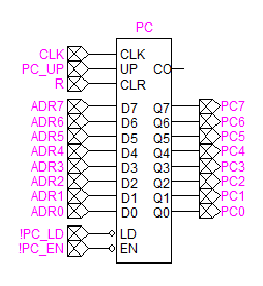
\includegraphics[scale=0.6]
  {content/figures/Blockschaltbild-programm-counter.png}
  \caption{Blockschaltbild des Programm Counters}
  \label{fig:blockschaltbild-pc}
\end{figure}

Der Programm Counter zählt die Adressen der Opeationen hoch, die ausgeführt werden. Dabei geht eine 8 bit Adresse in den Counter und ebenfalls wird eine 8 bit Adresse ausgegeben.


\subsection{Adress Register}
\label{sec: adress-register}

Besteht aus zwei 2x4 Multiplexern, besteht aus zwei 2x4 Adressbits, werden für den RAM verwendet

\subsection{Operations Register}
\label{sec: operations-register}

Das Operationsregister (OpReg) speichert einen 4-Bit-Wert und verwendet dazu die Eingangssignale WriteOp und RAM3..0.

Das Signal WriteOp wird vom Steuerwerk bereitgestellt, während RAM3..0 aus dem RAM kommt. Im Fetch-Zustand ist RAM3..0 der aktuelle Befehl, während es in anderen Zuständen auch Daten oder Teile einer Adresse sein kann.

WriteOp hat die Aufgabe, die aktuell ausgeführte Operation über den Fetch-Zustand hinaus zu speichern und verfügbar zu machen. Mithilfe eines Multiplexers entscheidet WriteOp, ob ein neuer Wert aus RAM3..0 ins Register geschrieben wird oder der bereits gespeicherte Wert erhalten bleibt:

WriteOp = 0: Der aktuell gespeicherte Wert wird bei der nächsten aktiven Flanke erneut übernommen und beibehalten.
WriteOp = 1: Der Wert von RAM3..0 wird bei der nächsten aktiven Flanke in das Register geschrieben.
Diese Logik ermöglicht dem Operationsregister, bestehende Befehle über mehrere aktive Flanken hinweg zu speichern oder neue Befehle bei Bedarf aufzunehmen

\subsection{Steuerwerk}
\label{sec:steuerwerk}